\section{Architectural Write Latency Investigation}
\label{sec:brewrc-investigation} This section presents a series of
experiments that characterize the write latency behavior of commercial
ReRAM crossbar memories. By applying carefully selected test patterns
and analyzing the resulting write latency distributions, the memory
array word size, polarity serialization properties, and timing
perturbations due to embedded ECC functions are identified. These
results motivate and directly inform the BREW-RC technique presented in
Section~\ref{sec:brewrc-method}.

\subsection{Experiment I: Redundant Write Latency}
\label{sec:brewrc-exp1} In a crossbar-based architecture, the word size
of the memory array is the smallest unit that can be serialized through
the write path, and is therefore the natural choice for the ECC encoder
data word width $k$. The target memories allow 1--256\,B write
operations, but the physical word size is not disclosed in the device
specification. To infer $k$, the latency characteristics of redundant
write operations are used. A \emph{redundant write} reinforces the
existing logical state of ReRAM cells; because no transitions occur, the
write latency reflects the minimum $t_w$ and the fixed per-word
programming overhead of the controller. This makes redundant writes a
low-noise probe of write-path serialization granularity. Redundant
writes with burst sizes of 1--256\,B are performed on 10 randomly
selected 256\,B-aligned addresses. A 256\,B contiguous memory segment
$S$ is first programmed to a random initial state. For each byte
position $i_B$ within $S$, an $i_B$-byte redundant write is performed.
\begin{figure}[t!]
    \centering
    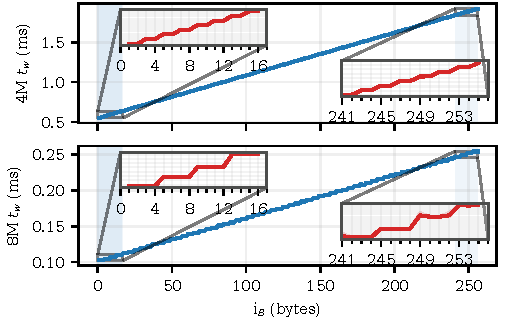
\includegraphics[width=0.95\linewidth]{fig/images/pdf/redundant-bytes-lineplots.pdf}
    \vspace{-.45cm}
    \caption{Write latency measurements ($t_w$) for $i$-byte redundant write operations on 4M (top) and 8M (bottom) devices.}
    % \vspace{-.65cm}
    % The aggregated redundant write times of four MB85AS4MT and four MB85AS8MT. All bursts are measured 10 times at 10 random 256B base addresses on each chip. All initial buffer data is randomized\, and each burst amount overwrites data redundantly from the base address up to the burst amount.}
    \label{fig:red-scan}
\end{figure}
Figure~\ref{fig:red-scan} shows the combined write latencies (mean and
shaded 95\% confidence interval) for all samples and test addresses. For
each 4M (8M) sample, $t_w$ overheads are accrued every two (four)
byte-lengths and show almost no variance, demonstrating that
serialization occurs on 2\,B (4\,B) boundaries. This result indicates
$k_{4M}=16$ bits and $k_{8M}=32$ bits, providing one dimension of the $k
	\times r$ parity submatrix.

\subsection{Experiment II: Single-Bit Transitions, Uniform Init}

\label{sec:brewrc-exp2}

Single-bit transitions may exhibit data-dependent $t_w$ if asymmetries
exist in the switching dynamics of the ReRAM cells or the PV loop. This
experiment characterizes single-bit write latency in uniformly
initialized 256\,B segments $S$, where all non-transitioning bits are
set to a uniform logical state. Each 256\,B span is initialized to
$S=\mathbf{0}$ (all zeros) or $S=\mathbf{1}$ (all ones). Each bit
position $i_b$ in the 2048-bit span is toggled 10 times in both logical
polarities and write latencies are captured. Because the minimum write
size in both memories is 1\,B, the byte offset and target bit are
computed from $i_b$ and two 1-byte write latency measurements are
performed.

\begin{figure}[h!]
    \centering
    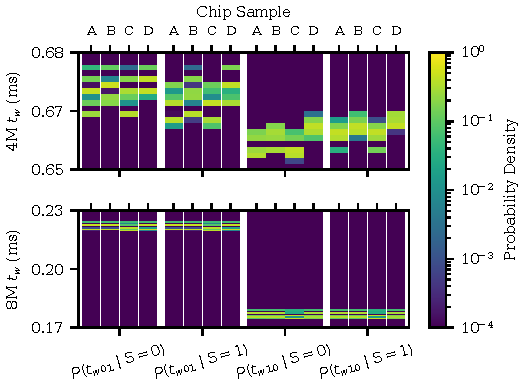
\includegraphics[width=0.95\linewidth]{fig/images/pdf/single-bit-buffer-scans-heat-bars.pdf}
    \vspace{-.5cm}
    \caption{Write latency distributions for 1-bit transitions within uniformly initialized 256-byte segments measured on 4 4M samples (top) and 4 8M samples (bottom). Each heatmap bar is a collapsed histogram colored according to the log-probability of observing a $t_w$ in each $\Delta t$-sized bin. $t_{w01}$ and $t_{w10}$ latencies correspond to data word transitions with a DHD of $\left(1,0 \right)$ and $\left(0,1\right)$, respectively. \label{fig:1b-buff-scan}}
\end{figure}

Figure~\ref{fig:1b-buff-scan} shows the resulting $t_w$ distributions
for each chip. Each bar represents a log-scaled collapsed histogram
combining all bit positions and addresses for one polarity, initial
state, and chip. For the 4M, write latency distributions for each
polarity overlap but are distinguishable. For the 8M, distributions for
each polarity are separated by a large margin. These relationships are
preserved across all samples of both devices, demonstrating that
single-bit transitions produce data-dependent write latency
distributions.

\subsection{Experiment III: Single-Bit Transitions, Non-Uniform Init}
\label{sec:brewrc-exp3} ECC parity bit transition polarities depend on
the state of the data word $d$. This experiment demonstrates that the
logical state of non-transitioning bits within the same word boundary
can influence the $t_w$ distribution of a transitioning bit, providing
evidence of parity bit activity. Ten 256\,B-aligned addresses are
randomly selected. From each address, a 256\,B span is initialized to
all zeros ($S=\mathbf{0}$). The first bit in each segment is designated
as the measurement bit. Before each measurement sequence, a contiguous
subset of neighboring bits extending from the measurement bit is
inverted ($S[1:i]=S'=\mathbf{1}$), creating a locally non-uniform
initial state. Each measurement bit is toggled 10 times per
configuration, with span sizes $i$ ranging from 1 to 2047 bits.
\begin{figure}[!h]
    \centering
    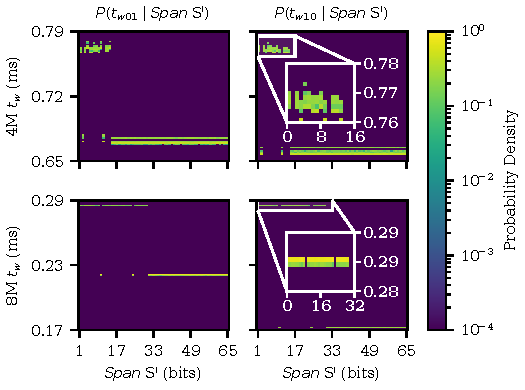
\includegraphics[width=0.95\linewidth]{fig/images/pdf/single-bit-sensitivity-scans-heat-bars-inset.pdf}
    \vspace{-.4cm}
    \caption{Write latency distributions for 1-bit $t_{w01}$ (left) and $t_{w10}$ (right) transitions within non-uniformly initialized 256-byte segments. Measurements from all 4 4M samples (top) and 4 8M samples (bottom) are aggregated. Each heatmap bar is a collapsed histogram colored according to the log-probability of observing a $t_w$ in each $\Delta t$-sized bin. The right plots zoom into the upper $t_w$ distributions to show 1-bit transitions that become \texttt{BIPOLAR} due to parity bit activity. \label{fig:sensitivity-scan}}
\end{figure}
The results are shown in Figure~\ref{fig:sensitivity-scan}. Two key
observations are made. First, beyond the word size established in
Experiment~I, the write latency distribution stabilizes: the influence
of neighboring bit states on write latency ends at the logical word
boundary. Second, while the span of $S'$ is smaller than the word
boundary, single-bit writes exhibit substantially longer latencies than
those observed under uniform initialization. These elevated latencies
are consistent with parity bit activity in the opposing polarity to the
transitioning data bit, causing codeword-level polarity serialization.

\subsection{Experiment IV: Single-Byte Transitions, Uniform Init}
\label{sec:brewrc-exp4} This experiment measures $t_w$ for all possible
($2^{16}$) single-byte transitions on all 4M and 8M samples, linking
write latency cluster membership to unipolar and bipolar codeword
transitions. This experiment is similar to the 1-byte latency
characterization performed in~\cite{tolga2024trng}, where the 4M device
was evaluated as an entropy source for TRNGs. It is repeated here with
one extension: the state of all inactive bytes in the word is varied,
setting them to either all 1s or all 0s, to exercise the full dataword.
For each chip, measurements are performed on 10 word-sized segments. To
suppress the effect of rare long-tailed latency events, the minimum
$t_w$ ($t_{wmin}$) is taken for each byte transition across all
segments.
\begin{figure}[t!]
    \centering
    \hspace{-0.75cm}
    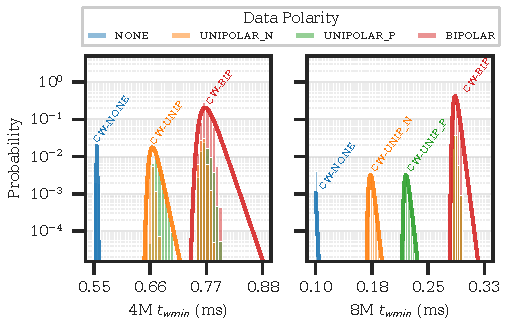
\includegraphics[width=0.95\columnwidth]{fig/images/pdf/sierpinski-clustering-mixture-curves.pdf}
    \vspace{-.45cm}
    \caption{4Mb and 8Mb $t_{wmin}$ measured for all 1-byte transitions. Histogram bars are colored according to data polarity. The curves correspond to EM-fitted mixture components that trace our observed latency clusters. We label each component according to our inferred codeword behavior \label{fig:sierp-hist}.}
    % \vspace{-.65cm}
\end{figure}
Figure~\ref{fig:sierp-hist} shows the results for the 4M and 8M. Three
unique $t_w$ distributions are observed for the 4M and four for the 8M.
The minimum $t_w$ distribution is exclusively occupied by redundant
write operations. Bipolar dataword transitions always occupy the highest
$t_w$ distribution. Unipolar dataword transitions occupy either an
intermediate $t_w$ distribution or the highest $t_w$ distribution. For
the 4M, unipolar transitions occupying the intermediate distribution
overlap. For the 8M, two distinct intermediate distributions exist, each
occupied by transitions of a single polarity. These observations are
consistent with~\cite{tolga2024trng}. The observation that certain
unipolar dataword transitions occupy the bipolar timing distribution
confirms that underlying parity bit activity modifies the codeword DHD,
causing polarity serialization. The cluster membership of each
transition is determined by the codeword DHD, not the dataword DHD
alone.
